\subsection{Força de senhas e cadeias de Markov}

\subsubsection{Descrição do problema e hipóteses probabilísticas}

Serviços online impõem políticas de senha, mas os usuários tendem a escolher senhas
com padrões previsíveis. Essa previsibilidade reduz o esforço necessário para
adivinhar uma senha, já que um atacante pode tentar primeiro as combinações mais
prováveis. O objetivo deste estudo é modelar a escolha de senhas por um processo
estocástico e quantificar a sua previsibilidade, comparando a incerteza do modelo
com a de uma senha totalmente aleatória.

A escolha de cada caractere é modelada por uma cadeia de Markov de ordem $2$, na qual
a probabilidade de um caractere depende apenas dos dois caracteres anteriores
\cite{ross2024models}. A primeira hipótese é que essa dependência de ordem $2$ resume
toda a informação relevante do passado. A segunda é que as probabilidades de
transição são estimadas a partir de uma amostra de treino e que cada caractere é
sorteado de forma condicionalmente independente dado o par anterior.

\subsubsection{Modelagem probabilística}

Cada senha é tratada como uma sequência de caracteres delimitada por marcadores de
início e de fim. A probabilidade de uma senha sob o modelo é o produto das
probabilidades de transição, conforme a Equação~\ref{eq:senha_prob}, em que $c_i$ é
o $i$-ésimo caractere e $P(c_i \mid c_{i-2}, c_{i-1})$ é a probabilidade estimada de
transição.

\begin{equation}
	P(\text{senha}) = \prod_{i=1}^{L} P(c_i \mid c_{i-2}, c_{i-1})
	\label{eq:senha_prob}
\end{equation}

A previsibilidade da distribuição de senhas é medida pela entropia, que representa a
incerteza média em bits. A entropia foi estimada por simulação de Monte Carlo,
gerando uma amostra de senhas pelo modelo e calculando a média do logaritmo de suas
probabilidades, conforme a Equação~\ref{eq:senha_entropia}, em que $M$ é o número de
senhas geradas.

\begin{equation}
	H \approx -\frac{1}{M} \sum_{m=1}^{M} \log_2 P(\text{senha}_m)
	\label{eq:senha_entropia}
\end{equation}

Esse valor é comparado com a entropia de uma senha de mesmo comprimento médio
composta por caracteres uniformemente aleatórios, igual a $L \log_2 26$ para um
alfabeto de $26$ letras. A diferença entre as duas entropias quantifica a perda de
aleatoriedade introduzida pelos padrões de escolha.

\subsubsection{Implementação em R}

A matriz de transição de ordem $2$ foi estimada a partir de uma lista sintética de
senhas comuns, com suavização de Laplace para evitar probabilidades nulas. Foram
geradas $5000$ senhas pelo modelo, cada uma construída caractere a caractere até o
sorteio do marcador de fim. O Listing~\ref{lst:senha_gera} mostra a estimação da
matriz e a geração das senhas.

\begin{lstlisting}[caption={Estimação da matriz de transição e geração das senhas.}, label={lst:senha_gera}]
cont <- array(alpha, dim = c(length(estados), length(estados), length(saidas)),
              dimnames = list(estados, estados, saidas))
for (w in treino) {
  w_ext <- c("^", "^", strsplit(w, "")[[1]], "$")
  for (i in seq_len(length(w_ext) - 2)) {
    cont[w_ext[i], w_ext[i + 1], w_ext[i + 2]] <-
      cont[w_ext[i], w_ext[i + 1], w_ext[i + 2]] + 1
  }
}
probs <- sweep(cont, 1:2, apply(cont, 1:2, sum), FUN = "/")
senhas <- replicate(5000, gerar_senha(probs))
\end{lstlisting}

\subsubsection{Resultados e interpretação}

As senhas geradas tiveram comprimento médio de $8{,}5$ caracteres. A entropia
estimada do modelo foi de $26{,}5$ bits, enquanto a entropia de uma senha aleatória
de mesmo comprimento seria de $40{,}0$ bits. A diferença de cerca de $13{,}5$ bits
indica que o espaço efetivo de busca de um atacante que conhece os padrões é muito
menor que o espaço de força bruta, da ordem de milhares de vezes.

A Figura~\ref{fig:senhas_logprob} mostra a distribuição do logaritmo da
probabilidade das senhas geradas. A concentração de massa próxima dos valores mais
altos revela que muitas senhas são bastante prováveis sob o modelo, enquanto a longa
cauda à esquerda reúne senhas raras. Essa assimetria é a base da vantagem do
atacante, que ordena suas tentativas pelas senhas mais prováveis.

\begin{figure}[H]
	\centering
	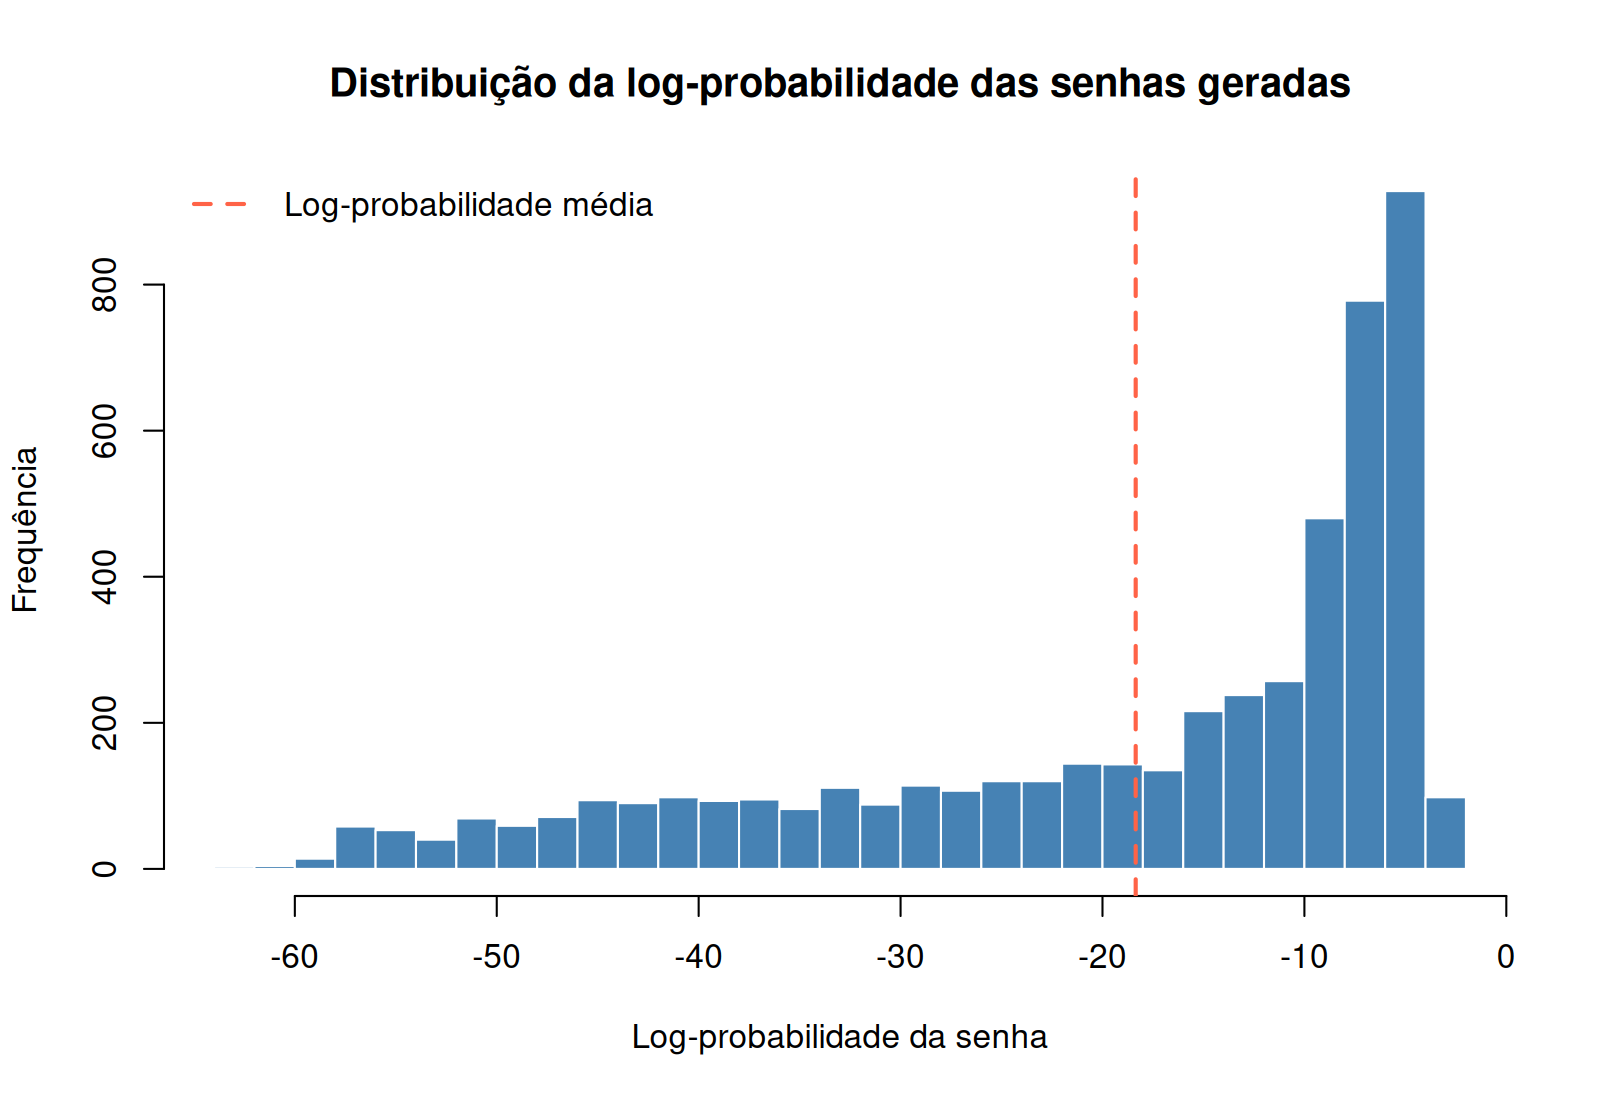
\includegraphics[width=0.8\textwidth]{secoes/07_atividade_integradora/atv_4/imagens/fig_senhas_logprob.png}
	\caption{Distribuição do logaritmo da probabilidade das senhas geradas pelo modelo.}
	\label{fig:senhas_logprob}
\end{figure}

A hipótese de Markov de ordem $2$ não elimina a dependência entre caracteres, mas a
limita ao par anterior, o que captura padrões frequentes do idioma e reproduz a
previsibilidade real das senhas. A simulação permite quantificar essa previsibilidade
sem percorrer analiticamente o espaço de todas as sequências possíveis, que é grande
demais para ser tratado de forma direta.
